%Carthage Physics Senior Thesis
%Author: Aaron Scheets

\documentclass[twocolumn,12pth]{article}
\usepackage[hmargin={1.25in,0.75in},bmargin=1in,tmargin=1in]{geometry} 
\usepackage{setspace}
\usepackage{url}
\usepackage{syntonly}
\usepackage[ampersand]{easylist}

\usepackage{natbib}

\usepackage{amsmath}
\usepackage{mathtools}
\usepackage{gensymb}
\usepackage{amssymb}
\usepackage{float}
\providecommand{\e}[1]{\ensuremath{\times 10^{#1}}}

\usepackage{graphicx}
\usepackage{caption}


\title{Writing A Fluid Solver From First}

\author{Aaron Scheets}

\onecolumn

\begin{document}

\maketitle

\section{Components of a Numerical Solution}




\subsection{Discretization Method}

Numerical solutions are approximations to continuous mathematical expressions.
The mathematical expressions of interest in this case are the component equations of the set of Navier-Stokes equations.
These are equations in space, and in time. 
In the realm of mathematical analysis, and when we solve equations analytically, we deal with continuous functions.
When equations cannot be solved analytically, as is the case with the Navier-Stokes equations, they can be approximated through \textit{discretization methods}.
Discretization method solutions are approximations because they can only produce information about the function at a finite set of points.
The process of discretization leaves our mathematical model as a system of linear equations or as a system of ordinary differential equations.
Now our mathematical model can be solved by solving a linear system of equations, which depending on the size of the fluid application, involves performing a massive amount of arithmetic operations.
This is convenient if you are using a computer because computers are really good at solving massive amounts of arithmetic operations.
Before the advent of computers, the Navier-Stokes equations could be solved using similar discretization methods, however, this required rooms full of people solving linear systems of equations to get a final answer.
The discretization process is essentially chopping up: 1.The fluid domain (the pipe), into a set of finite points, and 2.The mathematical model (the Navier-Stokes Equations) into a set of finite arithmetic operations.

The fluid domain \textit{discretized} into a set of finite points is known as a \textit{Numerical Grid}.
Numerical grids can be uniform or non-uniform; in general it is easier to solve for a uniform, structured grid, see Figure \ref{fig:grid}.
This is the type of grid I used to represent the pipe in the simulation.

\begin{figure}
\centering
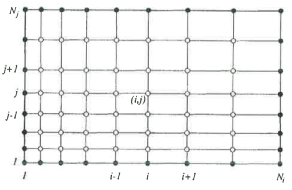
\includegraphics[width=3.0in]{numericalGrid.png}
\captionof{figure}{To solve for the velocity and pressure of water flowing within the pipe, first we need to divide the pipe into a finite set of points. We are interested in the value of velocity and pressure at these points.}
\label{fig:grid}
\end{figure}

\subsubsection{Finite Differences}

Finite difference methods are an approximation to the derivative.
Given some function $u(x)$, if we are interested in the derivative of $u(x)$ at some point $i$ along the x-axis, we could approximate the derivative as follows:

\begin{equation}
\frac{du}{dx} = \frac{u(i + \Delta{x}) - u(i)}{\Delta{x}}
\label{eq:FD}
\end{equation}

This gives the rate of change in $u$ with respect to $x$.
This particular approximation is a \textit{forward approximation} because we are approximating the derivative at $i$ by considering values of $u$ in the forward direction.
The \textit{backwards approximation} is a similar expression, but we are taking the derivative with respect to points to the left of $i$ on the x-axis.

\begin{equation}
\frac{du}{dx} = \frac{u(i) - u(i - \Delta{x})}{\Delta{x}}
\label{eq:BD}
\end{equation}

A central difference about the point $i$ would be observing the change in $u$ from $i - \Delta{x}$ to $i + \Delta{x}$:

\begin{equation}
\frac{du}{dx} = \frac{u(i + \Delta{x}) - u(i - \Delta{x})}{2\Delta{x}}
\label{eq:CD}
\end{equation}

\begin{figure}
\centering
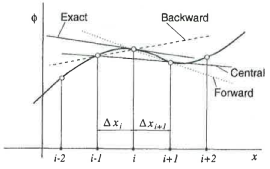
\includegraphics[width=3.0in]{finiteDif.png}
\captionof{figure}{The forward, backward and central differences are approximations to the actual derivative of our function. Some approximations will be better than others, depending on the function in consideration.}
\label{fig:difs}
\end{figure}

The factor of $2\Delta{x}$ in the central difference comes about beause we are observing the change in $u$ over twice the distance utilized in the forward and backward difference equations.

\subsubsection{Finite Difference from Taylor Series}
If we want to be a little more specific in our expression for the forward, backward, central differences, we can express them using the Taylor Series.
The Taylor Series expansion of our function $u(x)$ centered at the point $i$ is the following:

\begin{equation}
u(x) = u(x_i) + (x-x_i)\bigg(\frac{\partial{u}}{\partial{x}}\bigg)_i + \frac{(x-x_i)^2}{2}\bigg(\frac{\partial^2{u}}{\partial{x^2}}\bigg)_i + \frac{(x-x_i)^3}{6}\bigg(\frac{\partial^3{u}}{\partial{x^3}}\bigg)_i + ... + \frac{(x-x_i)^n}{n!}\bigg(\frac{\partial^n{u}}{\partial{x^n}}\bigg)_i + H 
\end{equation}

The $H$ in our expression stands for the \textit{higher order terms}, the product of the higher order derivatives and the displacement between $x$ and $i$.
Thus we can solve for the first derivative of $u$ with respect to $x$, $(\frac{\partial{u}}{\partial{x}})_i$:

\begin{equation}
\bigg(\frac{\partial{u}}{\partial{x}}\bigg)_i = \frac{u(x) - u(i)}{x-i}
- \frac{(x-i)^2}{2}\bigg(\frac{\partial^2{u}}{\partial{x^2}}\bigg)_i - \frac{(x-i)^3}{6}\bigg(\frac{\partial^3{u}}{\partial{x^3}}\bigg)_i - ... - \frac{(x-i)^n}{n!}\bigg(\frac{\partial^n{u}}{\partial{x^n}}\bigg)_i + H 
\end{equation}

If $x$ is sufficiently close to $i$, the higher order terms will tend to zero and we can be satisfied with the following expression, which is a \textit{first order approximation} to the derivative of $u$ with respect to $x$ at the point $i$:

\begin{equation}
\bigg(\frac{\partial{u}}{\partial{x}}\bigg)_i \approx \frac{u(x) - u(x_i)}{x-x_i}
\end{equation}

Returning to our numerical grid, if we keep our expansion centered at the point $x_i$ and let $x = x_{i+1}$, our Taylor Series Expansion becomes:

\begin{equation}
u(x_{i+1}) = u(x_{i}) + (x_{i+1}-x_{i})\bigg(\frac{\partial{u}}{\partial{x}}\bigg)_i + \frac{(x_{i+1}-x_{i})^2}{2}\bigg(\frac{\partial^2{u}}{\partial{x^2}}\bigg)_i + \frac{(x_{i+1}-x_{i})^3}{6}\bigg(\frac{\partial^3{u}}{\partial{x^3}}\bigg)_i + ... + \frac{(x_{i+1}-x_{i})^n}{n!}\bigg(\frac{\partial^n{u}}{\partial{x^n}}\bigg)_i + H 
\end{equation}

Solving for $(\frac{\partial{u}}{\partial{x}})_i$  we have an expression equivalent to the forward difference derivative we found above (\ref{eq:FD}):

\begin{equation}
\bigg(\frac{\partial{u}}{\partial{x}}\bigg)_i \approx \frac{u(x_{i+1}) - u(x_i)}{\Delta{x}}
\end{equation}

So, we have found our forward difference equation concretely, that is, we have the first order approximation and knowledge of the higher order terms as well.
The higher order terms that we dropped will eventually be a source of error that we will have to keep track of later. 
By applying the above process to the pairs of points $x_i$ and $x_{i-1}$, as well as $x_{i+1}$ and $x_{i-1}$ we can obtain the backward difference formula and central difference formula, respectively, from the Taylor Series Expansion.

\begin{equation}
\bigg(\frac{\partial{u}}{\partial{x}}\bigg)_i \approx \frac{u(x_{i}) - u(x_{i-1})}{\Delta{x}}
\end{equation}

\begin{equation}
\bigg(\frac{\partial{u}}{\partial{x}}\bigg)_i \approx \frac{u(x_{i+1}) - u(x_{i-1})}{x_{i+1}-x_{i-1}}
\end{equation}

\subsubsection{Finite Difference: Second Derivative}

Coming soon...


\end{document}

